\subsection{Principe du fonctionnement de Netfilter}
%% - firewall\\
%% - flot de paquets.\\
%% - insertion de notre programme dans le flot.\\
%% 2 schémas : \\
%% - PacketFlow.png \cite{l7}\\
%% - schema1.png


L'architecture de Netfilter peut se résumer à une série d'accroches
(\og hooks \fg{}) qui permettent de brancher des modules de traitement de
paquets IP à divers endroits le long de leur transit à travers la pile
réseau du noyau, comme détaillé sur la fig \ref{NF}. Sur cette figure,
les paquets arrivent en 1 après avoir passé quelques tests
élémentaires de sanité (checksum IP correct, etc\ldots).

\begin{figure}[h]
  \begin{center}
    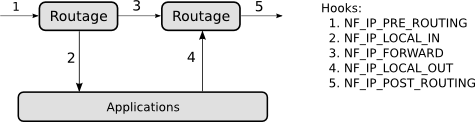
\includegraphics{netfilter.png}
    \caption{Architecture de Netfilter pour l'IPv4}
    \label{NF}
  \end{center}
\end{figure}

Sur chacune de ces accroches on peut venir brancher des fonctions pour
modifier ou filter les paquets. Chaque fonction ainsi branchée est
assortie d'une priorité qui détermine dans quel ordre les fonctions
sont appelées sur les paquets. Les fonctions standardes utilisées dans
le noyau implémentent le filtrage et la modification de paquets
(iptables), ainsi que le suivi de connections (conntrack).

Iptables consiste un ensemble de règles de filtrage ou de modification
de paquets regroupés en \textit{tables}. Celles-ci sont consultées
lors du passage par certaines accroches.

\begin{center}
  \begin{tabular}{|l|l|}
    \hline
    \textbf{Table} & \textbf{Accroches} \\
    \hline
    filter & NF\_IP\_LOCAL\_IN, NF\_IP\_LOCAL\_OUT, NF\_IP\_FORWARD \\
    \hline
    nat & NF\_IP\_PRE\_ROUTING, NF\_IP\_POST\_ROUTING \\
    \hline
    mangle & Toutes \\
    \hline
  \end{tabular}
\end{center}

La table \textit{filter} regroupe les règles traditionnelles d'un
firewall comme accepter, rejeter ou ignorer des paquets IP selon
certains critères. La table \textit{nat} regroupe des règles de
modification à la volée de la source ou de la destination d'un
paquet. Enfin la table \textit{mangle} regroupe des règles de
modification des autres entêtes IP ou TCP. Iptables est facilement
extensible par d'autres modules noyau, ce qui permet de définir de
nouvelles règles et de nouveaux critères.

Le suivi de connections, en première approche, identifie les flux en
fonctions des triplets IP source, port source et port de
destination. Le fait d'implementer ce suivi dans un module séparé
permet de réutiliser ces informations dans d'autres parties du
noyau. Ainsi avec le module \textit{state} de iptables, on peut ainsi
filter un paquet selon qu'il appartienne à un flux déjà connu
(ESTABLISHED) ou s'il initie un nouveau (NEW). Le module conntrack est
également capable de suivre certains protocoles qui utilisent
plusieurs flux comme FTP ou IRC. Dans le module \textit{state}, de
tels flux sont marqués RELATED.

\subsection{Études des possibilités pour développer un module Netfilter}
%% Description des deux possibilités existantes :\\
%% - faire un module noyau ;\\
%% - faire un programme userspace.\\\

%% Comparaison point à point de ces deux solutions et justification de notre choix.

Pour développer un module de filtrage applicatif pour Netfilter il
existe deux approches possibles. Le projet \textit{L7-filter}
\cite{l7} développe d'ailleurs les deux.

La première possibilité est de coder une extension d'iptables sous
forme d'un module noyau. Ceci présente l'avantage d'être très rapide
puisqu'on a directement accès au pointeur de paquet de la couche
réseau ce qui nous évite d'avoir à faire des copies intégrales du
paquet. En revanche, le développement est plus difficile puisque nous
sommes limités au langage C et aux librairies du noyau. Dans notre cas
ceci est particulièrement problématique puisque nous souhaiterions
pouvoir utiliser des expressions régulières pour identifier des URL ou
des noms de fichiers, et donc pouvoir utiliser une librairie de
gestion des expressions régulières. Dans le cas du module noyau de
\textit{l7-filter}, le choix a été d'intégrer au module une librairie
d'expressions régulières allégée mais pas vraiment très
standarde. Enfin un bug ou une faille de sécurité dans un module noyau
peut compromettre ou crasher la machine sur laquelle il tourne.

A contrario, il est possible d'utiliser la cible NFQUEUE de Netfilter
pour déléguer le traitement d'un paquet à un programme userspace. Cela
peut se faire à n'importe quelle accroche Netfilter au moyen de règles
\textit{iptables} adaptées. Ceci pénalise inévitablement les
performances du traitement puisqu'il faut copier la totalité du paquet
de la mémoire noyau vers la mémoire userspace et vice
versa. Cependant, les avantages en termes de développement sont
considérables puisqu'il est possible d'utiliser du C++ et des
librairies d'expressions régulières complètes et standardes. Par
ailleurs, un plantage du programme userspace n'entraînera pas tout le
système avec lui.

Nous avons opté pour la deuxième solution. En particulier, dans
l'optique d'un boîtier filtrant, notre programme récupérera des
paquets à partir de la table \textit{filter} au niveau de l'accroche
\textit{FORWARD} et y appliquera éventuellement une marque. Cette
marque servira à prendre une décision au niveau de l'accroche
\textit{POSTROUTING} dans la table \textit{mangle}. Ceci est
schématisé sur la figure \ref{schema1}.

\begin{figure}[h]
  \begin{center}
    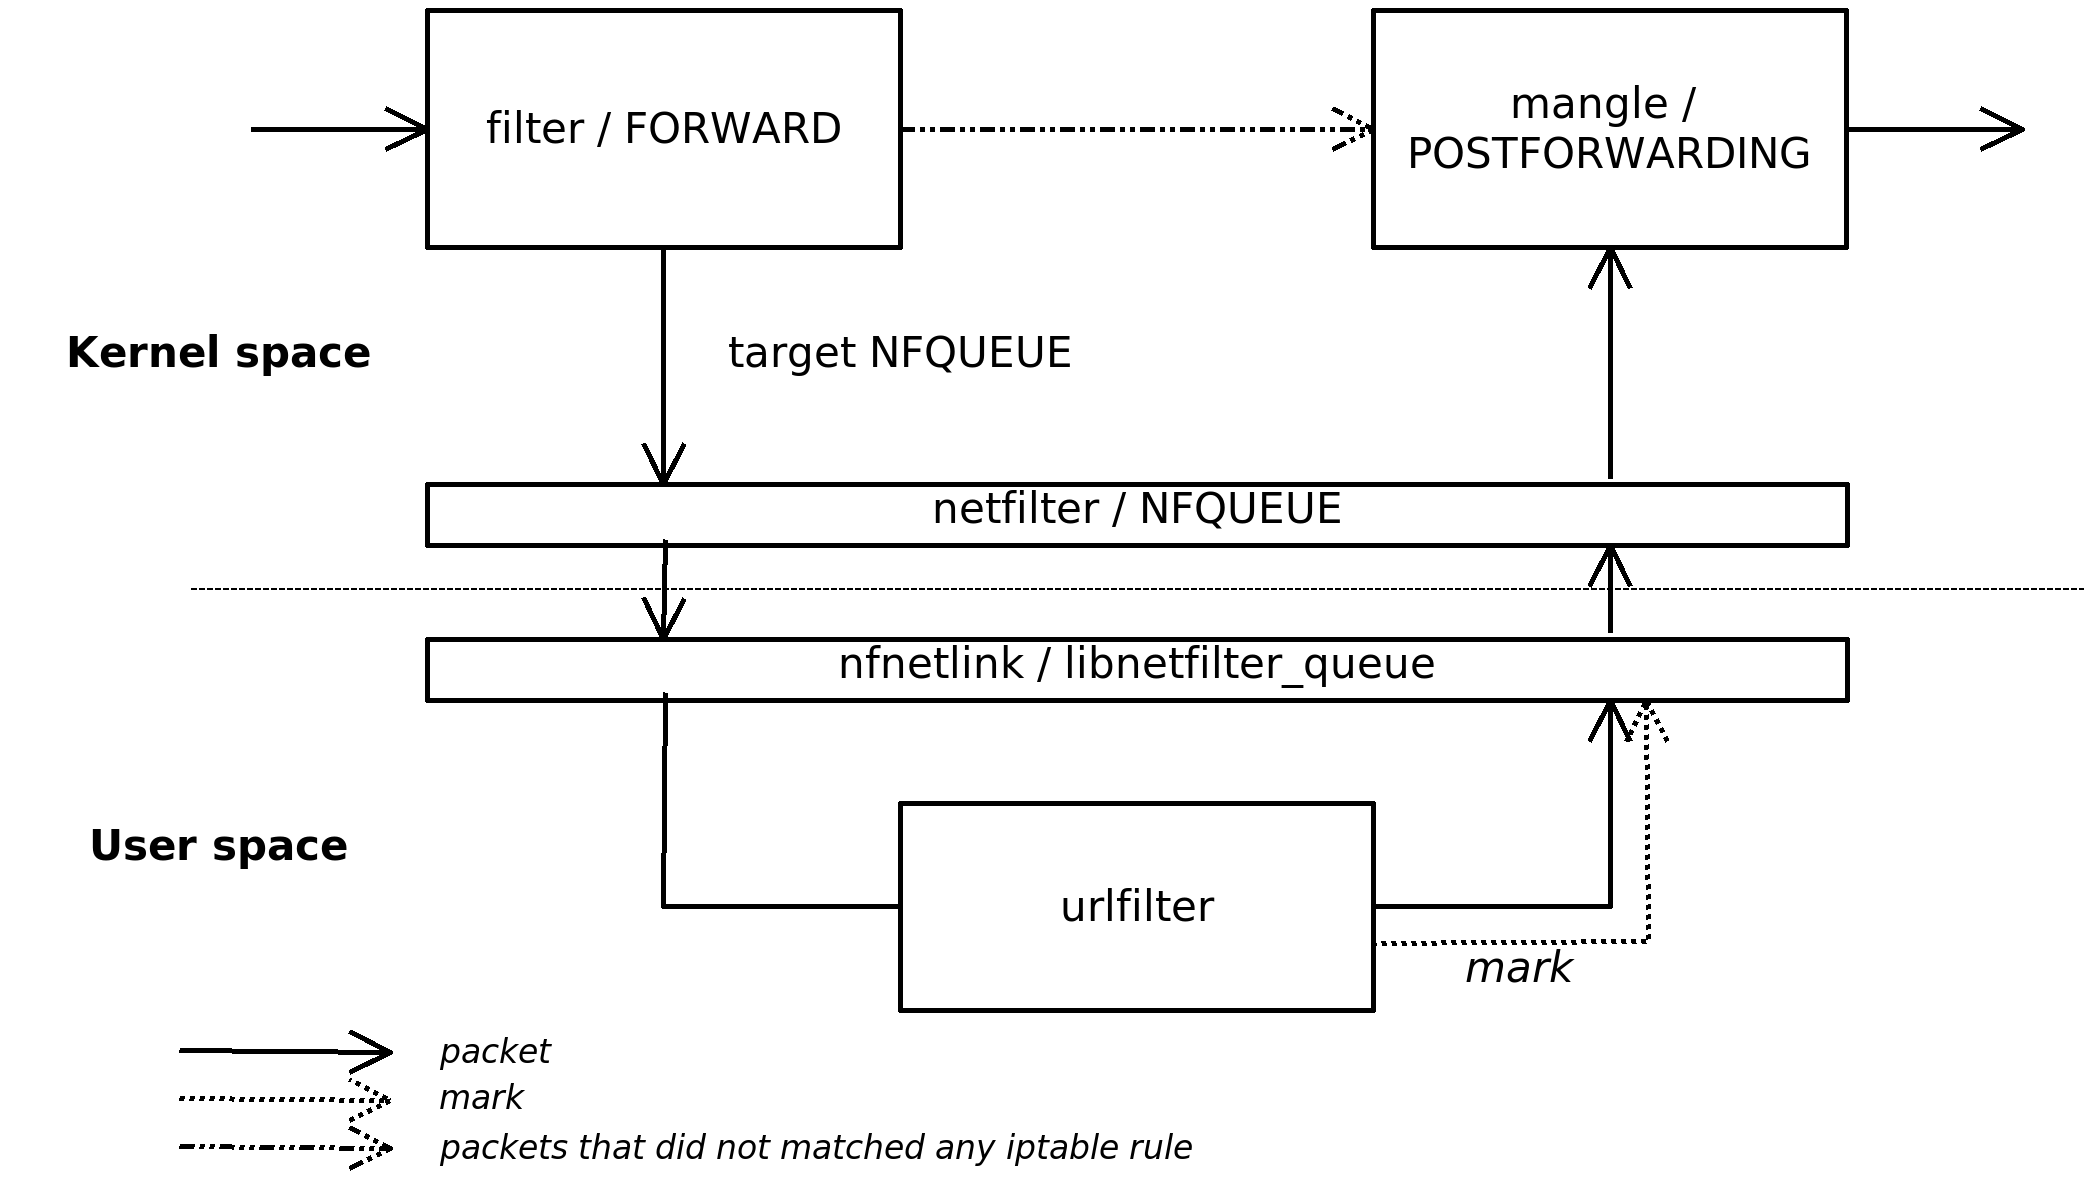
\includegraphics[scale=0.2]{schema1.png}
    \caption{Interaction entre Netfilter et notre filtre applicatif}
    \label{schema1}
  \end{center}
\end{figure}
